% ---------------------------------------------------------------
% Blown trailing edge -- one-page result sheet.
% GENERATED by make_actB_sheet.py; every number is substituted from the
% theory module, none is typed by hand.  Edit the generator, not this file.
% ---------------------------------------------------------------
\documentclass[8pt,a4paper]{extarticle}
\usepackage[margin=10mm,top=8mm,bottom=6mm]{geometry}
\usepackage{booktabs,graphicx,xcolor,caption,microtype,multicol}
\setlength{\columnsep}{8mm}
\usepackage[T1]{fontenc}
\usepackage{lmodern}
\definecolor{navy}{HTML}{1F4E79}
\definecolor{boxbg}{HTML}{FBF6E9}
\definecolor{boxrule}{HTML}{C9A227}
\captionsetup{font=small,labelfont=bf,skip=3pt}
\setlength{\parindent}{0pt}
\setlength{\parskip}{1pt}
\pagestyle{empty}

\newcommand{\shead}[1]{\vspace{1pt}{\color{navy}\bfseries\large #1}\vspace{1pt}\hrule\vspace{3pt}}
\newcommand{\role}[1]{{\color{navy}\bfseries #1.}}

\begin{document}

{\color{navy}\LARGE\bfseries Blown trailing edge: how much lift does the jet buy?}\\[2pt]
{Two-dimensional aerofoil section, jet blown from the trailing edge at
$\tau = 30^\circ$ below the chord line, $\alpha = 0^\circ$,
chord Reynolds number $1.0 \times 10^{6}$, chord $1.0$~m, free stream $10.0$~m\,s$^{-1}$.}

\shead{The answer in one line}

Lift does not grow in proportion to blowing. It grows as the \emph{square
root} of the jet momentum coefficient $C_\mu$, so the first increment of blowing
is worth far more than the last: the first $0.05$ of $C_\mu$ buys 8.47 of
lift coefficient per unit $C_\mu$, the last $0.20$ only 1.95 --- a factor
of 4.3. Sizing a blowing system on a straight line through a
low-blowing data point overpredicts the lift at $C_\mu = 0.40$ by
169\%.

\shead{Table 1 -- Published thin-aerofoil theory for a jet-flapped section}

\begin{center}\small
\begin{tabular}{cccccc}
\toprule
Jet momentum & Total lift & \multicolumn{2}{c}{of which:} & Marginal lift & Uncertainty \\
coefficient & coefficient & jet reaction & pressure lift & per unit $C_\mu$ & on the value \\
$C_\mu$ [--] & $(C_L)_\infty$ [--] & $C_\mu \sin(\tau+\alpha)$ [--] & [--] &
$\mathrm{d}C_L/\mathrm{d}C_\mu$ [--] & [--] \\
\midrule
0.00 & $0$ & $0$ & $0$ & --- & $<10^{-9}$ \\
0.05 & $4.23403 \times 10^{-1}$ & $2.50000 \times 10^{-2}$ & $3.98403 \times 10^{-1}$ & 4.331 & $<10^{-9}$ \\
0.10 & $6.04776 \times 10^{-1}$ & $5.00000 \times 10^{-2}$ & $5.54776 \times 10^{-1}$ & 3.131 & $<10^{-9}$ \\
0.20 & $8.68742 \times 10^{-1}$ & $1.00000 \times 10^{-1}$ & $7.68742 \times 10^{-1}$ & 2.294 & $<10^{-9}$ \\
0.40 & $1.25948 \times 10^{0}$ & $2.00000 \times 10^{-1}$ & $1.05948 \times 10^{0}$ & 1.716 & $<10^{-9}$ \\
\bottomrule
\end{tabular}
\end{center}

\vspace{-7pt}
{\footnotesize The jet-reaction column is the direct vertical component of the
jet momentum, reported separately and never folded silently into the lift
column: here it is a \emph{part} of the total, and the pressure-lift column is
what remains. The marginal column is the slope of the total with respect to
$C_\mu$; it is unbounded as $C_\mu \to 0$, which is the square-root law stated as
a number. Uncertainty is the arithmetic error of evaluating the published
expression; the accuracy of the published fit is not stated in the source.}

\shead{Table 2 -- Solved flow field: four blown conditions and a slot-closed reference}

\begin{center}\small
\begin{tabular}{ccccccc}
\toprule
Jet momentum & Lift from the & Jet reaction & Lift, surface & Movement in the & Turbulence & Difference \\
coefficient & aerofoil surface & (added, not & $+$ jet reaction & last 4{,}000 & equation & from \\
$C_\mu$ [--] & $C_{L,\mathrm{surface}}$ [--] & measured) [--] & [--] & iterations [--] & imbalance [--] & Table 1 [\%] \\
\midrule
0.00$^{\dagger}$ & $5.50595 \times 10^{-5}$ & $0$ & $5.50595 \times 10^{-5}$ & $7 \times 10^{-7}$ & $3.46 \times 10^{-6}$ & --- \\
0.05 & $4.05733 \times 10^{-1}$ & $2.50000 \times 10^{-2}$ & $4.30733 \times 10^{-1}$ & $5 \times 10^{-7}$ & $5.94 \times 10^{-6}$ & +1.73 \\
0.10 & $5.48846 \times 10^{-1}$ & $5.00000 \times 10^{-2}$ & $5.98846 \times 10^{-1}$ & $7 \times 10^{-7}$ & $2.55 \times 10^{-5}$ & -0.98 \\
0.20 & $7.43999 \times 10^{-1}$ & $1.00000 \times 10^{-1}$ & $8.43999 \times 10^{-1}$ & $4 \times 10^{-5}$ & $4.57 \times 10^{-5}$ & -2.85 \\
0.40 & $1.00999 \times 10^{0}$ & $2.00000 \times 10^{-1}$ & $1.20999 \times 10^{0}$ & $8 \times 10^{-6}$ & $1.47 \times 10^{-4}$ & -3.93 \\
\bottomrule
\end{tabular}
\end{center}

\vspace{-7pt}
{\footnotesize The surface column integrates pressure and shear over the
aerofoil only; it does \emph{not} contain the jet reaction, which is added
explicitly in the fourth column to give a quantity comparable with Table~1.
``Movement'' is how much the lift still shifted over the final 4{,}000
iterations: half the range it covered there, rounded up to one significant
figure. ``Turbulence equation imbalance'' is how far the turbulent kinetic
energy equation is from being satisfied at the last iteration; the target set
before running was $1 \times 10^{-6}$. $^{\dagger}$The $C_\mu = 0$ row is a
reference case with the slot \emph{closed}; the other four have it open and
differ only in jet strength.}

\vspace{2pt}
\begin{center}
\begin{minipage}[t]{0.455\textwidth}
\vspace{0pt}
\centering
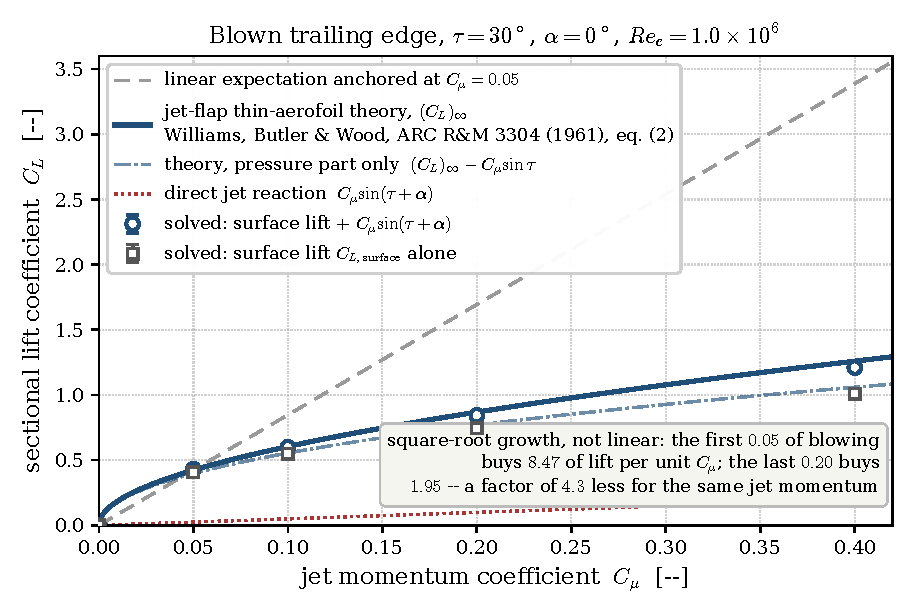
\includegraphics[width=\textwidth]{fig_lift_vs_blowing.pdf}

\vspace{2pt}
{\footnotesize\raggedright\textbf{Figure 1. Lift against blowing.} The solid
curve is published thin-aerofoil theory for a jet-flapped section (Williams,
Butler \& Wood, ARC R\&M 3304, 1961, eq.~2). The dashed grey line is what a
linear expectation anchored at $C_\mu = 0.05$ would have predicted; the gap
between the two is the message of this sheet. Uncertainty bars on the solved
points are the movement column of Table~2 and are smaller than the markers.\par}
\end{minipage}\hfill
\begin{minipage}[t]{0.515\textwidth}
\vspace{0pt}
\setlength{\fboxsep}{6pt}
\fcolorbox{boxrule}{boxbg}{\parbox{\dimexpr\textwidth-14pt}{\footnotesize%
{\bfseries Please read before using these numbers.}\\[2pt]
$\bullet$ The theory curve is trustworthy arithmetic against a published
formula. The solved points are not yet finished calculations and none of them is
described here as verified.\\
$\bullet$ The uncertainty column in Table~2 says how much each number was still
moving at the end of the run. It is \emph{not} a total error bar: the
contribution from mesh resolution has not been established for these five
conditions, and it is larger than the number shown.\\
$\bullet$ The published formula is an interpolation fit to computed values, valid
for blowing from the trailing edge with no separate flap, and is used whole over
the range it was fitted for. It is inviscid thin-aerofoil theory: no stall, no
separation, no viscous loss, so it overstates lift wherever the real jet sheet or
boundary layer breaks down.\\
$\bullet$ Everything here is two-dimensional. No finite-span correction has been
applied, and a real wing of finite aspect ratio will achieve less.
}}

\vspace{5pt}
{\color{navy}\bfseries What this cost}\vspace{1pt}\hrule\vspace{2pt}
{\footnotesize\raggedright The five solved conditions used
117.5 core-minutes of compute in total
(23.8, 24.4, 21.8, 22.3, 25.2 core-minutes respectively).
The figure quoted before any of them started was 56.8
core-minutes, so the work came in 2.07 times the upfront estimate. The
sixth, finer-mesh companion condition was quoted at
90.5 core-minutes upfront and used
98.7, 1.09 times its estimate. The theory curve
costs no solver time. At the machine's hourly rate of
\$0.0513 per core-hour that is \$0.100 spent
against a \$0.049 estimate for the five, and \$0.084 against
\$0.077 for the finer mesh. Money figures are derived from the hourly
rate; they are not read from a metered bill.\par}
\end{minipage}
\end{center}

\shead{What has been checked, what has not, and how the team reads it}

\begin{multicols}{2}
\textbf{Checked.} The theory curve reproduces the published expression exactly.
The lift derivatives were read off the printed page of Williams, Butler \& Wood,
\emph{The Aerodynamics of Jet Flaps}, Aeronautical Research Council Reports and
Memoranda No.~3304 (H.M.S.O., 1963), page~5, equation~(2), and the jet-reaction
convention $C_\mu \sin(\tau + \alpha)$ off page~3. Our evaluation reproduces the
values fixed before running to better than $5 \times 10^{-10}$ in lift
coefficient at every point in Table~1, and the marginal-lift column matches an
independent finite-difference evaluation of the same expression to eight figures.

\textbf{Checked.} The reference section, slot closed, returns a surface lift
coefficient of $5.51 \times 10^{-5}$ at zero incidence, as a
symmetric section must. The same solver and reader gave $1.01$ at the strongest
blowing, so the near-zero is physics, not a reader that could only give zero.

\textbf{Not checked.} \emph{None of the solved points in Table~2 is offered as
verified against anything.} The solutions are still tightening: no condition has
brought every equation below the $1 \times 10^{-6}$ target set before running,
and no mesh-refinement study has been completed for these five conditions. The
last column of Table~2 is an observation, not an agreement claim.

\role{Lead Researcher} The physics worth taking away is the square-root law:
blowing buys circulation, and circulation grows with the square root of jet
momentum, so the system pays back fastest at low blowing rates. At
$C_\mu = 0.40$ the jet provides $0.20$ of lift coefficient directly and
1.06 indirectly, through the pressure field it induces on
the aerofoil --- five times the direct part, and that amplification is the
point of the configuration.

\role{Lead Engineer} Size the system at the knee, not at the top. Going from
$C_\mu = 0$ to $0.05$ delivers 0.42 of lift coefficient;
quadrupling jet momentum from $0.10$ to $0.40$ delivers only another
0.65. Budget analysis time accordingly:
this flow becomes markedly harder to solve as blowing increases, so a strongly
blown case is not a mildly blown case with a different inlet number.

\role{Lead Numericist} Confidence differs sharply between the two tables.
Table~1 is arithmetic against a published expression, exact to the digits shown.
Table~2 has not reached the target set before running: the turbulence equation
imbalance grows monotonically with blowing, from $3.46 \times 10^{-6}$ at the reference
to $1.47 \times 10^{-4}$ at the strongest jet, a factor of 43. The lift is
still moving at the end of every run, by the amount in the movement column,
which is why that column is quoted at all --- a settling indicator is not a
converged one. In every one of the five conditions the solver also had to clip
the turbulence energy back to zero wherever it went negative, on
81 to 97\% of iterations and continuously
through the final one, so these fields are held non-negative by that clipping
rather than converged free of it; on the companion mesh it is
99\%. The finer companion mesh has completed,
and it does not close the mesh question: it is a different grid topology on a
different reference area, run as a diagnostic, so it is not a refinement of the
five and no grid-refinement study has been carried out. The mesh contribution
to the uncertainty on Table~2 therefore remains unquantified.
\end{multicols}

\shead{Figure notes}

\begin{multicols}{2}
\role{The section} Two-dimensional wing section, 1.0~m chord, symmetric, at
zero incidence in a 10.0~m\,s$^{-1}$ stream, with a 5.0~mm slot at the
trailing edge blowing a sheet of air 30$^\circ$ below the chord line. $C_\mu$
is the jet's momentum divided by the oncoming stream's dynamic pressure times
the chord. Because the section is symmetric at zero incidence it makes no lift
at all without blowing.

\role{Lift against blowing} All five conditions share one grid of 39\,984
cells. The four blown ones differ from one another only in how hard the slot
blows, so differences among those four are caused by the blowing and nothing
else; the fifth is a reference with the slot closed, and is not the same wing
with the jet turned down to zero. The first 0.05 of jet momentum buys a
disproportionate share of the lift, which is the square-root law read off the
chart.

\role{The flow picture} Red is air moving faster than the oncoming stream,
blue slower, and white the same speed, with the dashed contour marking exactly
the oncoming speed. The dark line traces the fast sheet leaving the slot; it
bends the oncoming flow downward, and that bending is what lifts the wing,
there being no hinged flap anywhere in the model. Contours and streamlines are
drawn on a display grid for legibility, while every number quoted on this sheet
is read from the solver's own output.

\role{Where the sheet goes} The slot aims the sheet 30$^\circ$ below the
chord line and the oncoming flow turns it, so it travels well above where a
free jet of the same angle would go. That turning is the force: the jet pushes
the air down and the air pushes the jet, and the wing, up. The trace stops
where the sheet can no longer be told apart from the surrounding air and is not
extrapolated beyond it.
\end{multicols}

\end{document}
